\documentclass[a4paper,12pt]{article}
\usepackage[english]{babel}
\usepackage[utf8]{inputenc}

%
% For alternative styles, see the biblatex manual:
% http://mirrors.ctan.org/macros/latex/contrib/biblatex/doc/biblatex.pdf
%
% The 'verbose' family of styles produces full citations in footnotes, 
% with and a variety of options for ibidem abbreviations.
%
\usepackage{graphicx}
\usepackage{csquotes}
\usepackage[style=verbose-ibid,backend=bibtex]{biblatex}
\bibliography{sample}

\title{Markovian Approach to Positive-only Problems}

\author{Shayan Amani}

\begin{document}
\maketitle

\section{Preliminaries}

\section{Bounding}
We can use available inequalities to bound our solution. We are always interested in finding upperbound for the policies or solution we propose. Hence, by applying those inequalities -based on requirements of each of them- the upper-bound can be found. Confidence intervals come into the problem where the results are bounded with an upper-bound. Moreover, confidence intervals are authentic measures of reliability of a solution.

    \subsection{Markov's Inequality}
The most simplistic inequality among the other described here in terms of being realxed about the constraints and requirements. The only requirement that needs to be satisfied is $X \geq 0$.
\begin{equation}
\mathrm {P}(X \geq a ) \leq \frac { \mathrm { E}( X ) } { a }
\end{equation}

    \subsection{Chebyshev's Inequality}
    \subsection{Chernoff bound}


\section{Methodology}


\section{Case Study}
The current case is a study on an invasive plant (non-native to the ecosystem) in New England area, namely glossy buckthorn [capitalization?].


\section{Bayesian Settings}
Sampling using a logistic regression (or any other methods) we can generate some distributions for our features (bio10 and bio5 REVIEW and alpha) then we are able to feed these to a linear program to calculate weights (L1 norm or any other distance metrics) and then we can build our ambiguity set based on what we get as weights.

% 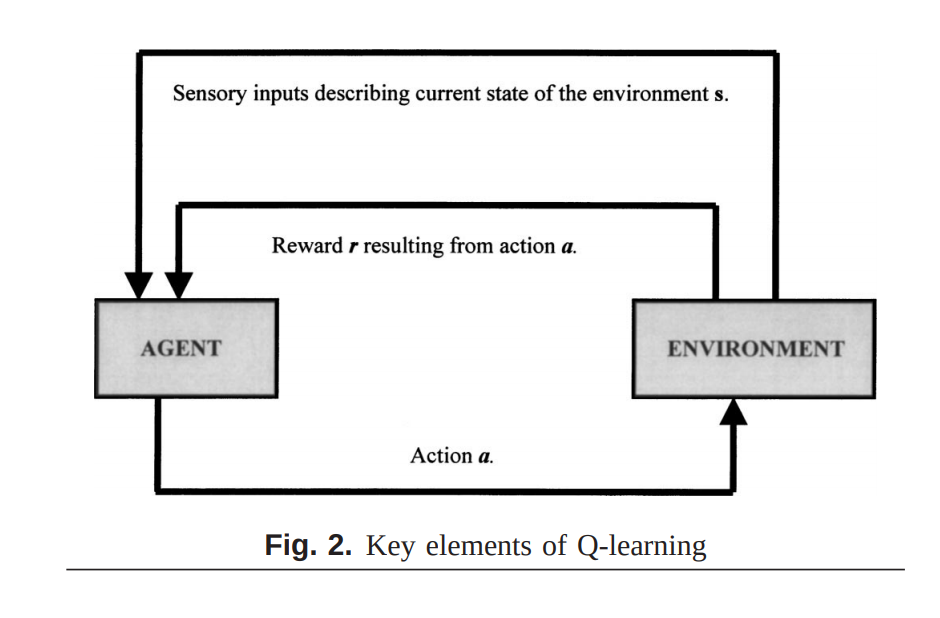
\includegraphics[width=1\columnwidth]{elements.png}

\section{A/B Test vs. Multi-armed Bandit Problem}
In a multi-armed bandit problem agent choose and pull one of the arms randomly at the beginning. The pulled arm bandit generates a distribution with specific values of mean $\mu_i$ and variance. The distribution is stationary but still unknown before pulling. \autocite{\autocite{brassard}}

\begin{tabular}{|c|c|}
    \hline
    \textbf{A/B test}    &   \textbf{Multi-armed bandit}  \\
    \hline
    \hline
    pure exploration    &   exploration along with exploitation \\
    \hline
    return after completion &   immediate return while running \\
    \hline
    expensive   &   cost-efficient \\
    \hline
\end{tabular}

\subsubsection{Upper Confidence Bound Algorithm}
Upper confidence interval includes true expected value and it gets narrow down (becomes smaller) after each iteration of the algorithm. In other words, the agent becomes more assured about the return value as it runs through each iterations. The agent picks the next upper confidence interval to exploit and continue with that until it finds a new higher value. Unneeded to mention that the two main actor in this algorithm are as follows:
\begin{itemize}
    \item Confidence interval becomes tighter along with iterations
    \item Return value along iterations converges to the expected true value.
\end{itemize}


% This is an example citation \autocite{ginsberg}.
% \lipsum[1] % dummy text

% This is another example citation \autocite{brassard}.
% \lipsum[2] % dummy text

% This is a repeated citation \autocite{brassard}.
% \lipsum[3] % dummy text

% This is another example citation \autocite{adorf}.
% \lipsum[4] % dummy text 

\end{document}